\documentclass[11pt]{article}

\usepackage[utf8]{inputenc}
\usepackage[english]{babel}
\usepackage{graphicx}
\usepackage[margin=1in]{geometry}
\usepackage[parfill]{parskip}
\usepackage{listings}
\usepackage{color}
\usepackage{float}
\usepackage{tocloft}
\usepackage{url}


\title{LPHY1300 Personal project report :\\ Simulation of a particle detector}
\author{\textsc{Schils} Arnaud\\ \textsc{Lardinois} Simon}
\date{2015-2016}

\begin{document}

	\lstset{language=C++,
	captionpos=b,
	frame=single,
	                basicstyle=\ttfamily,
	                keywordstyle=\color{blue}\ttfamily,
	                stringstyle=\color{red}\ttfamily,
	                commentstyle=\color{green}\ttfamily,
	                morecomment=[l][\color{magenta}]{\#}
	}
\maketitle

\newpage


\renewcommand\cftsecleader{\cftdotfill{\cftdotsep}}
\renewcommand{\contentsname}{Table of contents}
\tableofcontents


\newpage
\section*{Introduction}

	Nowadays, the huge amount of computing power offered by modern computer systems allows
	to solve complex scientific problems numerically. The art of solving physics problems using
	computers is referred as \textit{computational physics}. This modern field
	is multidisciplinary: it brings together applied mathematics,
	computer science and physics. It offers a third way to do physics
	that supplements theory and experiment.

	In this thesis, these numerical techniques are applied to the field of particle
	detectors physics. In order to design the best detectors,
	physicists have to know the measured signal resulting from the passage of a particle
	in the detector. Unfortunately, due to the complex geometries of these detectors
	and the various physical phenomena to handle, this signal is not easy
	to compute analytically.

	This is why, in the context of this thesis, a software  to compute the current measured
	by a particle detector due to the passage of a particle has been developed.
	This software has then been used to study silicon and gas particle detectors.

	% In the context of our lesson LPHY1300 personal project, we
	% had to simulate a particle detector using the finite elements method. We
	% thus develop our program "pdetect" which simulates the electric potential
	% and electric field inside a pixel detector. It also computes the electric
	% current induce by an incident particle with a given trajectory.

	\subsection*{Overview of the contributions}

		The primary contribution of this thesis is the development of a C++ numerical software performing the
		following tasks.

		Firstly, it computes the potential and the electric field
		at each point of a particle detector solving the Laplace equation for non-trivial
		two-dimensions geometries. Three types of 2D detector geometries are supported.
		The Laplace equation is solved using the \textit{finite element method} with an adaptive
		grid refinement strategy. The software supports multithreading and therefore
		uses all available CPUs to quickly solve this equation.

		Secondly, the software computes the current resulting from the passage of a particle
		in the detector using the \textit{Shockley–Ramo theorem} and the solution of the
		computed electric field. Every possible particle trajectories in the detector
		are supported. Effects such as the \textit{mobility} difference between holes and
		electrons, the \textit{saturation} phenomena and the \textit{Townsend Avalanche}
		are handled.

		This software has been developed following the object-oriented
		programming paradigm and with the \textit{model-view-controller}
		software engineering pattern in mind. Thanks to the quality of the software
		architecture further extensions such as 3D geometries, additional physical effects or
		detector types and the support of distributed computations on clusters are possible
		without the burden of reimplementing an entire new software.

		The secondary contribution of this thesis is the use of this software to study
		the gas and silicon detectors. Finally, the results provided by the
		software have been compared with the results of \textit{Weightfield}~\cite{Cenna2015}, a
		software performing similar computations.

		%To perform this task, the software places charges
		%resulting from the ionization of the molecules inside the detector. Then, these
		%charges drift following the applied potential at the anode and cathode of the detector

	\subsection*{Organization of the thesis}

	This thesis is organized in six Sections. The remainder of this manuscript
is structured as follows.

		\begin{itemize}
			\item Section 1 introduces the finite element method and the
			C++ finite element library \texttt{deal.ii}. Then, \textit{Weightfield},
			a software simulating particle detectors, is presented.
			\item Section 2 is a resume of the detector physics concepts that must be
			known to understand the problem solved by the software developed in the
			context of this thesis.
			\item Section 3 presents the features of the software and the actions
			it performs in chronological order.
			\item Section 4 explains the software architecture and the role played by
			the most important classes.
			\item Section 5 presents the results obtained with our software for
			different set of parameters which models various detectors.
			\item Section 6 discusses the future work.
		\end{itemize}

		% In this paper we will first introduce briefly what the finite elements
		% method is, and then a library we used in our program, "deal.II".
		% After what we will explain properly our program, the way it works, and
		% also comparing our results with the results of "weightfield", another
		% simulator of a particle detector, already use in many experiences.
		% To finish this paper we will talk about two specific cases of detector,
		% a silicon detector, and a helium detector.


\section{Background and related work}

	This section is composed of three parts. Firstly,
	the finite element method is briefly explained. Then \textit{deal.ii},
	a C++ library implementing the finite element method is introduced. Finally,
	\textit{Weightfield}, another software performing particle detector simulation,
	is presented.

	\subsection{Finite element method}

		The finite element method is a numerical technique for
		finding approximate solutions to boundary value problems for partial
		differential equations. The finite element method subdivides a large
		problem into smaller, simpler, parts, called finite elements. The
		simple equations that model these finite elements are then assembled
		into a larger system of equations that models the entire problem. It
		then uses variational methods from the calculus of variations to
		approximate a solution by minimizing an associated error function.

	\subsection{Deal.II library}

		In order to avoid to reinvent the wheel, it was decided to use the deal.ii library
		to solve the Laplace equation~\cite{Bangerth:2007:DGO:1268776.1268779}. This decision allows to rely on the optimized
		and robust code of deal.ii and to benefit from the cutting edge numerical methods this library provides.

		deal.II is a C++ library allowing to solve partial differential equations
		using the finite element method. It is a very powerful but low-level library.
		It offers several features such as adaptive meshes, grid handling
		and refinement, handling of degrees of freedom, input of meshes and output of results in
		graphics formats. Furthermore, deal.ii allows to easily write code that works
		for any dimensions because code using deal.ii is written independently of the space
		dimension. Thanks to this design choice, the code of our software is quite easily
		extensible to 3D.

		Finally, deal.ii supports multithreading as well as \textit{MPI~\footnote{Message
		Passing Interface. MPI is used to develop distributed softwares running on top of
		clusters of computers.}}. Therefore,
		deal.ii is able to hardness the power of multithreaded CPUs as well as
		clusters composed of hundreds of computers. Consequently,
		the software developed in this thesis is multithreaded and could be extended to
		exploit the resources offered by clusters.


	\subsection{Weightfield}

		Weightfield is a program to study the performance of silicon and diamond
		detectors~\cite{Cenna2015}. It simulates the energy released by particles in the detector
		and uses the Ramo's theorem to compute the signal current.

		Among others, Weightfield allows to play with the following parameters:
		sensor geometry, internal gain, doping of silicon sensor and its operating
		conditions, the application of a magnetic field, the ambient temperature and
		thermal diffusion.

		Weightfield has been used in this thesis to compare and valid the results
		obtained with our own software.

\section{Introduction to the physics of particle detectors}

	\label{equations}

	In this section, the concepts of particle detectors physics used in this project
	are introduced.

	A particle detector is composed of a cathode, an anode and an active media
	between them (gas,...). A potential difference is applied between the cathode
	and the anode~\cite{lphy2236}.

	When a particle pass through the active media, the radiation ionizes the media
	molecules along the particle trajectory.
	Because of the applied potential difference,
	produced ion-electron pairs drift inside the detector until they reach the anode
	(for the ions) or the cathode (for the electrons). These ions and electrons
	are moving charges and therefore produce a current.

	The number of ion-hole pairs per length $n_{eff}$ produced in the media by the
	particle passage is given by the following formula:

	\[n_{eff} = \frac{dE/dx}{w} \]

	where $dE/dx$ is the energy deposited by the particle in the media by
	unit of length, and $w$ is the average energy to produce one ion-pair.

	The charges drift in the detector media with a velocity function of the electric
	field and the mobility~\cite{spieler2005semiconductor}:

	\begin{equation}
		\vec{v} = \mu \vec{E}
		\label{eq:charge_speed}
	\end{equation}

	where $\mu$ is the \textit{mobility}. Electrons and holes (or ions) have different
	mobilities. For example, in Silicon, mobilities are 1350 and 450 $cm^2V^{-1}s^{-1}$,
	respectively. In gas, the mobility difference between electrons and holes is
	much larger, electrons are typically a thousand times faster ($\mu =$ 100 $cm^2V^{-1}s^{-1}$
	for electrons and $\mu =$ 0.1 $cm^2V^{-1}s^{-1}$ for holes). Notice that the mobility
	is not a constant in general.

	Due to saturation, the mobility decreases when fields of 104 $V cm^{-1}$ and higher are applied in
	the detector following the relation:

	\begin{equation}
		\mu_s = \mu \left (1 + \left (\frac{\mu |E_y|}{v_{sat}} \right )^{\beta} \right )^{-\frac{1}{\beta}}
		\label{eq:saturation}
	\end{equation}

	where $\beta$ is a constant, $\mu$ the mobility when not considering saturation,
	$E_y$ the component of the electric field along the axis orthogonal to the anode and cathode
	and $v_{sat}$ the saturation velocity. The saturation velocity depends on the
	media and the temperature.

	Once the velocity is known, the current generated by moving ion-electron
	pairs can be computed. The Shockley–Ramo theorem states that the instantaneous current generated
	by one moving charge $q$ at velocity $\vec{v}$ is:

	\begin{equation}
		i = -q \vec{v} \cdot \vec{E}_w
		\label{eq:ramo}
	\end{equation}

	where $q$ is the signed charge and $\vec{E}_w$ is the \textit{weighting field}. The weighting field is the electric field
	obtained when applying a potential of $1V$ to the measurement electrode and setting
	the potential of the other electrodes to $0V$.

	The instantaneous current measured
	by the detector is the sum of the currents generated by the holes and electrons:

	\begin{equation}
		i_{tot} = \sum_{holes} i_h + \sum_{electrons} i_e
		\label{eq:tot_current}
	\end{equation}

	An additional effect to take into account  when dealing with gas detectors is
	\textit{charge multiplication}~\cite{lphy2236}. This effect
	multiplies the primary ionization charges by an avalanche phenomena.
	The \textit{Townsend avalanche} is implemented in our software. It happens
	when the electric field is higher than $10^6Vm^{-1}$. The electrons collide
	with the molecules of the media and, if their kinetic energy is sufficient,
	extract additional electrons from this molecules.

	The Townsend avalanche multiplies the local number of electrons (and therefore the local electric
	charge) if the electric field is high enough and if the electrons are close
	to the cathode. When these conditions are fulfilled, during a time interval
	$\Delta t$ the initial electric charge $q_0$ is multiplied
	according to the formula:

	\begin{equation}
		q = q_0 e^{\alpha \Delta x}
		\label{eq:townsend}
	\end{equation}

	where $\Delta x$ is the distance covered by the electron and $\alpha$ the
	\textit{first Townsend coefficient}. This coefficient is computed as follows:

	\[\alpha = ap \ e^{-bp/E}\]

	where $a, b$ are constants depending on the gas media, $p$ the pressure in
	the detector (the atmospheric pressure is commonly used) and $E$ the norm
	of the electric field at the charges position.

\section{Software features}
\label{sec:features}

	This section first presents the features of the software. Firstly,
	the implemented detector geometries are presented. Secondly, some details
	about the resolution of the Laplace equation are provided. Thirdly, the
	computation of the current measured by the detector is described.

	The software handles three types of 2D geometries:

	\begin{enumerate}
		\item \texttt{Middle circular holes rectangle}: this geometry is a rectangle with circular
			holes vertically centered and uniformly distributed along the horizontal axis (see
			Figure~\ref{fig:mid_circle_geometry}). The configurable values of the geometry
			are the rectangle width,
			the hole radius, the inter holes centers distance and the number of holes.
			The potential is set to $0V$ at the top and bottom boundaries. Left and right
			boundaries have free boundary conditions.

		\begin{figure}[H]
		  \center
		  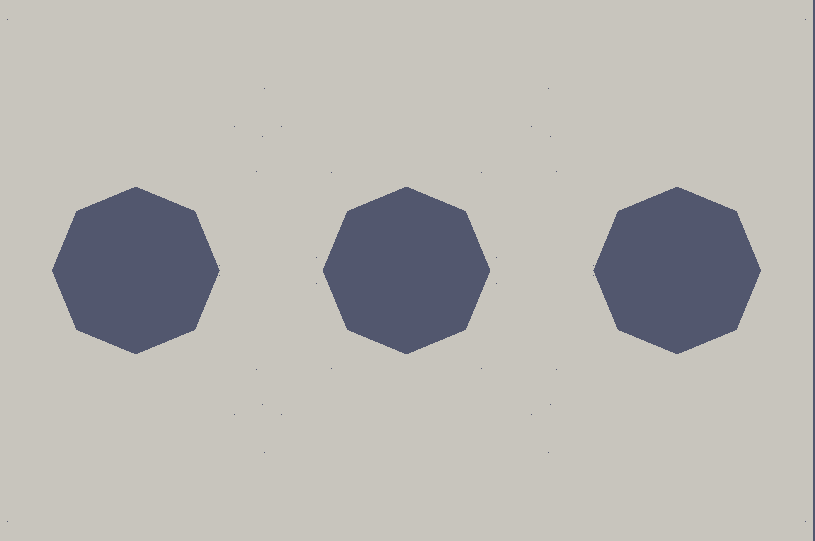
\includegraphics[scale=0.2]{images/detector_types/mid_circle_geometry.png}
		  \label{fig:mid_circle_geometry}
		  \caption{Middle circular holes rectangle geometry.}
		\end{figure}


		\item \texttt{Middle rectangular holes rectangle}: this geometry is a rectangle with rectangular
			holes vertically centered and uniformly distributed along the horizontal axis
			(see Figure~\ref{fig:mid_rect_geometry}).
			The configurable values of the geometry are the rectangle width, the number of
			holes, the inter holes distance, the hole width and the hole length.
			The potential is set to $0V$ at the top and bottom boundaries. Left and right
			boundaries have free boundary conditions.

		\begin{figure}[H]
		  \center
		  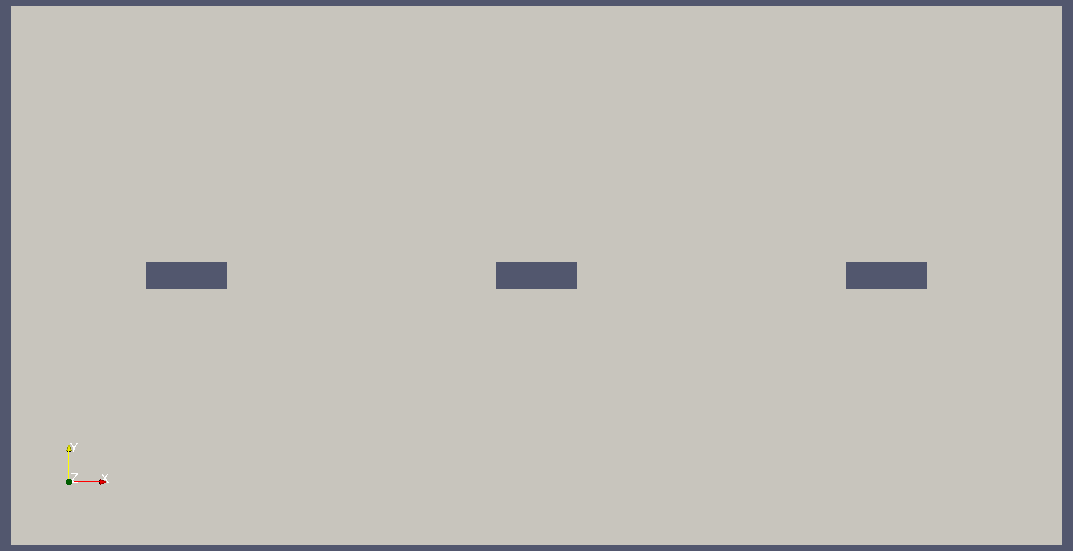
\includegraphics[scale=0.2]{images/detector_types/mid_rect_geometry.png}
		  \label{fig:mid_rect_geometry}
		  \caption{Middle rectangular holes rectangle geometry.}
		\end{figure}


		\item \texttt{Serrated rectangle}: this geometry is a rectangle with periodic
			holes inserted near the top boundary, along the horizontal axis
			(see Figure~\ref{fig:serrated_rect_geometry}).
			The configurable values of the geometry are the rectangle width, the number
			of holes, the hole length (i.e. the length of the side parallel to the top
			rectangle boundary), the hole width and the inter holes space.
			These holes are the potential sources, the boundary value at their borders is therefore
			the strip potential. The holes inter-spaces have free boundary conditions.
			The right and left boundaries of the rectangle have free boundary conditions as well.
			Finally, the value at the bottom boundary is 0V.

		\begin{figure}[H]
		  \center
		  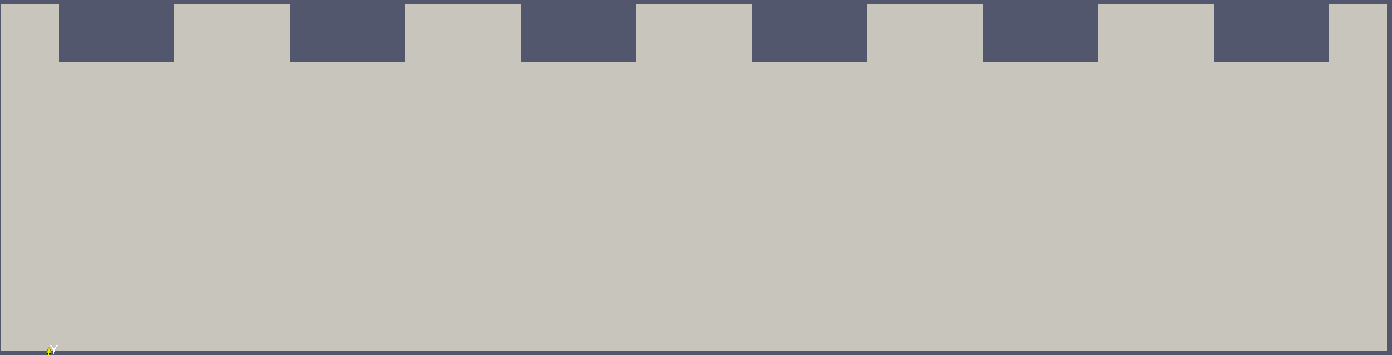
\includegraphics[scale=0.2]{images/detector_types/serrated_rect_geometry.png}
		  \label{fig:serrated_rect_geometry}
		  \caption{Serrated rectangle geometry.}
		\end{figure}

	\end{enumerate}


	For each one of these geometries, a coarse grid (or mesh) is generated using
	functions of the \texttt{deal.ii} library.

	Once the grid is generated (see Figure \ref{fig:no_refinement}), the Laplace equation is solved for the considered
	geometry. This is achieved using all available CPU cores and in several iterations.
	At the first one, the
	grid is coarse and the error on the computed results is high. Then, the grid is
	refined only at cells with the largest errors and the Laplace equation is
	solved on this denser grid. This process continues until
	the error is smaller than a relative error provided by the user at each cell of
	the grid (see Figure \ref{fig:high_refinement}). This is adaptive grid refinement. It allows to achieve good precision
	everywhere in the grid without losing time refining cells where the error is already small
	enough.

	\begin{figure}[H]
	  \center
	  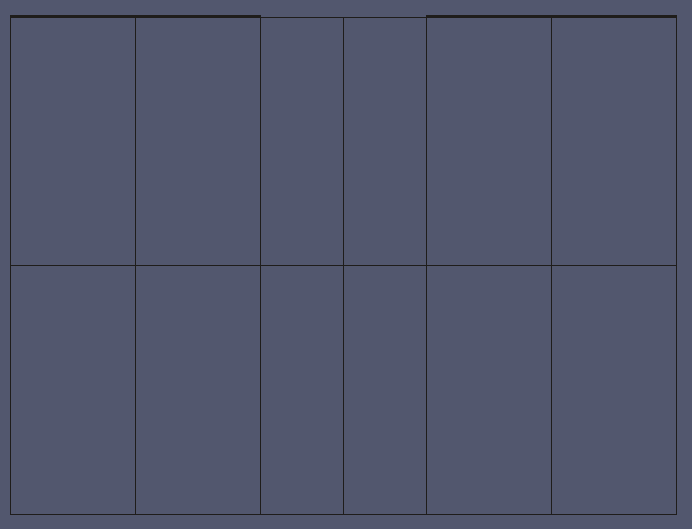
\includegraphics[scale=0.4]{images/grid_refinement/no_refinement.png}
		\caption{Example of initial grid. The initial grid should be as coarse as
		possible.}
	  \label{fig:no_refinement}
	\end{figure}

	\begin{figure}[H]
	  \center
	  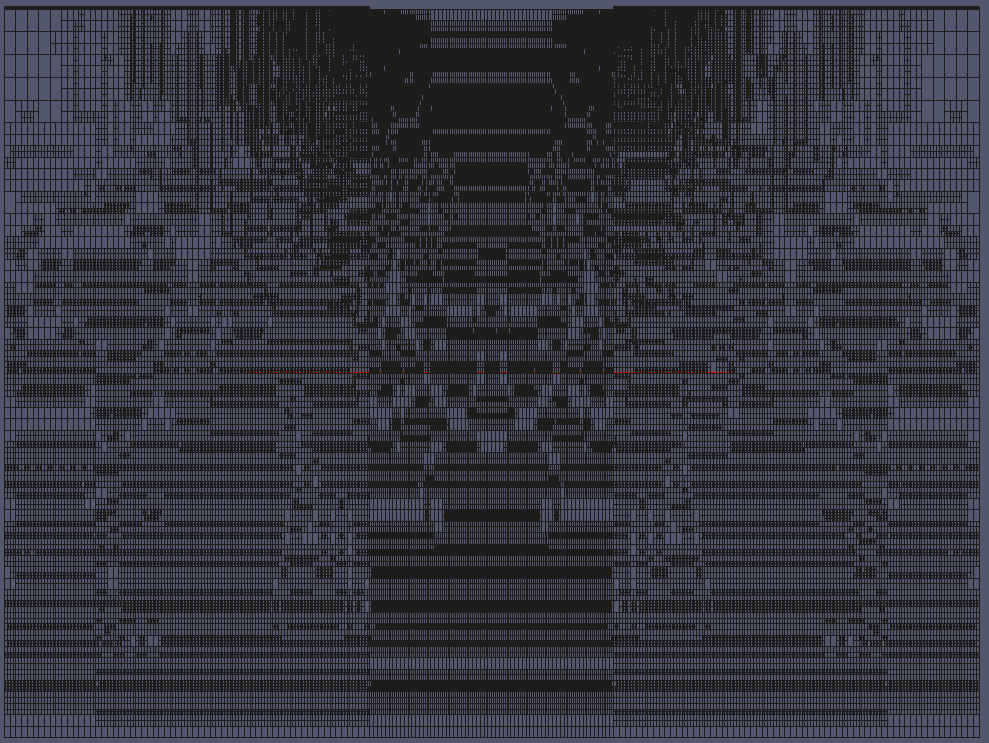
\includegraphics[scale=0.3]{images/grid_refinement/high_refinement.png}
	  \caption{State of the grid at the end of the adaptive grid refinement.}
		\label{fig:high_refinement}
	\end{figure}

	The result of the Laplace equation is of course the potential at each point of
	the grid. The gradient of the potential is available as well at
	the end of this process. A graphical representation of both the potential and
	its gradient can be written in a \texttt{vtk} file.
	These files can be read by the \texttt{Paraview} software.

	The same process is performed with different boundary conditions in order
	to compute the weighting potential and the weighting electric field.

	For each cell of the grid, the values of the potential, the error of the
	potential and the electric field are stored in a \texttt{rtree} data structure.
	In the algorithm computing the current measured by the detector, these three
	values have to be retrieved from the coordinates of a point. In order to retrieve the proper
	values, it is required to know to which cell the point belong. Since the grid
	is not uniformly refined, it is not easy to efficiently find this cell.
	Iterating through each cell of the grid is far too slow especially when 3D
	geometries will be introduced in the software. The algorithm finding the cell
	to which a point belong would have a $\mathcal{O}(n)$ time complexity, where $n$
	is the number of cells in the grid. The \texttt{rtree} data structure
	performs this search with a $\mathcal{O}(log(n))$ time complexity.

	The software then uses these results to compute the current measured by the
	detector. The user has to specify the particle trajectory. Any trajectory is
	supported. The computation of the current is composed of the following steps.

	Firstly, the ion-pairs generated by the particle pass are placed at their initial
	positions inside the detector. At this end, the intersections points between the
	detector boundaries and the particle
	trajectory are computed. Notice that a particle may enter and leave the detector
	several times (the potential sources, or strips, are not considered as being
	part of the detector). It happens for example if the particle trajectory is
	horizontal near the top boundary of a serrated rectangle geometry.
	The segments being part of both the particle trajectory and the detector
	geometry are retrieved. The total
	distance covered by the particle inside the detector is then computed as
	the sum of the length of these segments. From this, the total number of ions-pair
	created by the particle pass is computed
	as the product of the covered distance with the number of ions-pair created by unit
	of length. The number of ions-pair created by unit
	of length is considered as a constant and is different from one
	media to another. Depending on the precision level specified by the user, the
	total number of ions-pair
	is uniformly spread along the path covered by the particle inside the
	detector. When the precision is higher, the total number of pairs is spread
	among more points. On the opposite, if the precision level is set to 0,
	all ion-pairs are placed at the same point.


	Secondly, the charges are moved in the detector under the effect of the electric
	field. The speed of the charges is computed using Equation~\ref{eq:charge_speed}.
	Due to the saturation effect the mobility of charges may change depending on
	their position in the detector. Therefore, the mobility used in Equation~\ref{eq:charge_speed}
	is computed using Equation~\ref{eq:saturation} at each iteration.



	The new position of the charge is simply:

	\[(x',y') = (x + v_x \Delta t, \ y + v_y \Delta t)\]

	The time interval $\Delta t$ is automatically chosen by the software before
	each iteration depending on the maximum vertical speed of the charges:

	\[\Delta t = \frac{w}{v_{y_{max}} c}\]

	where $w$ is the detector width, $v_{y_{max}}$ the maximum vertical speed
	among all the charges moving inside the detector at the previous iteration and
	$c$ is a precision coefficient. This precision coefficient is a constant provided
	by the user. When the coefficient is greater, the time interval
	of the simulation is smaller and the results are more precise.
	Thanks to this adaptive $\Delta t$, the time interval is always sufficiently small.
	Using a constant $\Delta t$ may be a problem dealing with gas detector, because
	the mobilities of the hole and the electron differ greatly.

	For each time $t$, the current $i$ is computed using the Equations~\ref{eq:ramo}
	and~\ref{eq:tot_current}. Each pair $(t, i)$ is saved in a vector which can be
	written to a file at the end of the simulation.

	At the end of each iteration, the electric charge at one point in the detector
	may be multiplied due to the Townsend avalanche effect following Equation~\ref{eq:townsend}.
	Notice that this effect happens only for gas detectors.

\section{Software architecture}

	This software is developed in C++ with the object-oriented programming paradigm.
	This section firstly presents how the final software should be organized in several
	modules. Secondly, the most important classes and their responsibilities are
	presented. Relevant implementation details are also mentioned.

\subsection{Model–view–controller (MVC) software architectural pattern}

	The program main function calls functions from the \texttt{test} folder. These functions
	assemble the different objects to perform the required computation. In the
	final version of the program, functions of the test folder should be replaced
	by a graphic user interface: a \texttt{view} and a \texttt{controller} following
	the model-view-controller software engineering pattern. In this pattern code
	related to core of the program functionality (the \texttt{model}: mathematical computations, file access,...)
	is separated from the code related to the user interface (the \texttt{view}).
	The \texttt{view} and the
	\texttt{model} are connected by the \texttt{controller} module.

	The main advantage of this design pattern is to be able to change the user interface without
	performing any modification to the code of the \texttt{model} module. Furthermore,
	mixing model and graphic interface related code should be avoided because it leads to
	less readable and not modular code.

	The graphic user interface would allow the user to specify
	parameters of the simulation at runtime rather than hardcoding parameters
	directly in the functions of the \texttt{test} folder.
	The development of the \texttt{controller} and \texttt{view} modules
	is left for future work.

\subsection{The model module}

	The reminder of this section presents the most important classes
	included in the \texttt{model} module.



The \texttt{MyGridGenerator} class provides functions to generate \texttt{deal.ii}
grids (i.e. objects of type \texttt{Triangulation} handled by \texttt{deal.ii}) for supported
geometries. This class heavily relies on functions of the \texttt{deal.ii}
library. A common strategy is to first generate
little rectangles using the \lstinline{hyper_rectangle} method from the
\texttt{deal.ii GridGenerator} class and assemble them using the \lstinline{merge_triangulations}
method from the same class to obtain the desired grid. Developers led to build
methods to generate
new geometries must be aware that the \lstinline{merge_triangulations} method
requires the merged triangulations to have common vertices at the boundaries
where the two triangulations are adjacent, otherwise
the boundaries of the geometry may not be well defined, leading to strange behavior
when solving the Laplace equation.

	The \texttt{MyGeometryInfo} abstract class and provides informations
	related to the
	geometry of the detector as well as methods to compute the intersections of a
	line with the boundaries of the geometry and to check if a point is inside
	the geometry. This abstract class has three implementations: one for each
	geometry introduced at Section~\ref{sec:features}.

The \texttt{LaplaceSolver} class responsibility is to solve the Laplace equation.
The whole code related to finite element method resides in this class.
Its constructor is presented at Listing~\ref{lst:laplace_solv_constructor}.
\newline

\begin{lstlisting}[
	label=lst:laplace_solv_constructor,
	caption=Constructor of the \texttt{LaplaceSolver} class.]
LaplaceSolver(Triangulation<dim> *triangulation,
double refine_accuracy, unsigned max_iter, double stop_accuracy,
const Function<dim> *right_hand_side,
BoundaryConditions<dim> *boundary_conditions,
bool constraints_are_periodic)
\end{lstlisting}

The \texttt{triangulation} parameter is a pointer to a grid generated using methods of
the \texttt{MyGridGenerator} class. The \texttt{refine\_accuracy} is the maximum
error tolerated at each cell. For a given grid (fixed refinement level),
the \texttt{stop\_accuracy}  is a stop criteria that indicates if the solver has
reached convergence. If the error difference between two successive iterations
of the solver is less than \texttt{stop\_accuracy} the solver stopped iterating
on the current grid. Notice that it does not mean that the computation of the
Laplace solution is over: the solver may solve the equation on finer grids
afterwards until the error is less than \texttt{refine\_accuracy} everywhere
in the grid. The solver also stopped when the number of iteration on a given
grid is equel to \texttt{max\_iter}. The \texttt{right\_hand\_side} parameter
is the function $f$ at the right side of the Poisson equation:

\[\nabla^2 \phi(x,y) = f(x,y)\]

Since in this project the Laplace equation is solved, \texttt{right\_hand\_side}
simply refers to the trivial constant function $f(x,y) = 0$ for all $(x,y) \in R^2$.
The \texttt{boundary\_conditions} parameter is a function called by the Laplace
equation solver on each point of the domain boundary for which the free
boundary conditions are not enabled. Boundary values are encoded in this function.

The functions that dictates the boundary values are stored in the
\texttt{boundary\_conditions} folder. There are two functions for each
type of geometry: one provides boundary values fore the potential and the electric
field computation, the other one for the weighting potential and the weighting
electric field computation.

Finally, the \texttt{constraints\_are\_periodic} variable may be used to
enable or disable the free boundary conditions.

The core of the \texttt{LaplaceSolver} has been implemented based on the
\texttt{deal.ii} tutorial. The developer interested to extend the code of this
class (for example to enable computation on cluster) should refer to this
useful resource~\cite{deal.iituto}.

The results are retrieved from a \texttt{LaplaceSolver} object
 calling the \lstinline{void get_solution(Solution<dim> &sol)}
method with a properly allocated \texttt{Solution} object as parameter.
The results are encapsulated in a \texttt{Solution} object. Thanks to this
abstraction layer, it is possible to modify code in the class \texttt{LaplaceSolver}
or in the class \texttt{Solution} without having to change code in other
places in the program (as long as the interfaces of these classes are not
changed). For example it may be useful if one decides not to use \texttt{deal.ii}
anymore or if the data structure containing the results is changed.

The \texttt{Solution} class provides a method to access efficiently physical
quantities at any location in the grid as well as methods to output graphs
of the potential or the gradient of the potential. The physical quantities
are accessed efficiently thanks to the \texttt{rtree} data structure already
introduced in Section~\ref{sec:features}. The \texttt{rtree} implementation
used in this class is provided by the famous \texttt{boost} C++ library~\cite{boost.rtree}.
This implementation also supports 3D search spaces.

	The \texttt{Detector2D} class is an abstract class that models a detector
	represented by a two-dimensional geometry (a section of a detector). Implementation
	of this abstract class composes instances of the previously presented classes
	(\texttt{MyGeometryInfo}, \texttt{LaplaceSolver}, \texttt{BoundaryConditions}
	,...).

	Classes	implementing the \texttt{Detector2D} abstract class must implement the
	 following methods (much of them are already implemented in the \texttt{Detector2D}
	 class and are therefore common to all types of detector):
	\begin{itemize}
		\item \lstinline{void comp_potential()}: this method computes the potential
		at each point of the detector.
		\item \lstinline{void comp_weight_potential()}: this method computes the
		weighting potential	at each point of the detector.
		\item \lstinline{MyGeometryInfo* get_geometry_info()}: returns a pointer
		to a MyGeometryInfo containing all useful informations about the geometry
		of the detector.

		\item \lstinline{void get_solution(Solution<2> &sol)}: provides
		a \lstinline{Solution<2>} object allowing to retrieve the potential
		and the electric field at any point of the grid. Must be called
		after one call to \lstinline{void comp_potential()} with a properly instantiated
		\lstinline{Solution<2>} object as parameter.

		\item \lstinline{void get_solution_weight(Solution<2> &sol)}: provides
		a \lstinline{Solution<2>} object allowing to retrieve the weighting potential
		and the weighting electric field at any point of the grid. Must be called
		after one call to \lstinline{void comp_weight_potential()} with a properly instantiated
		\lstinline{Solution<2>} object as parameter.

		\item \lstinline{Hole get_hole()}: returns a \texttt{Hole} object having
		properties (mobility,...) corresponding to the type of the detector (helium, silicon).

		\item \lstinline{Electron get_electron()}: returns an \texttt{Electron} object having
		properties (mobility,...) corresponding to the type of the detector (helium, silicon).

		\item \lstinline{double get_hole_pairs_nbr_per_lgth()}: returns the number
		of ion-pairs per length generated by the particle pass in this
		type of detector (helium or silicon).

		\item \lstinline{double get_strip_potential()}: return the potential of
		the potential sources in the detector.

		\item \lstinline{double get_first_townsend_coefficient(Point<2> &pos, PhysicalValues<2> &values_at_pos)}:
		returns the first Townsend coefficient required to generate new ion-pairs due
		to the Townsend avalanche effect. For silicon detectors for which this effect
		does not apply, 0 is returned.

		\item \lstinline{virtual std::string params_to_string()}: returns a string
		containing the values of the most important parameters of the detector.

		\item \lstinline{void draw_vtk_graph_*}: this set of methods output some \texttt{vtk}
		files. These files contain a graphic representation of the potential and
		electric field. These files can be opened by the \texttt{Paraview} software.
	\end{itemize}

The last important class is the class \texttt{ElectrodeCurrent}. This class
is responsible of the computation of the current measured by the detector. Its
constructor is presented at Listing~\ref{lst:electrode_current_constructor}.
\newline

\begin{lstlisting}[
	label=lst:electrode_current_constructor,
	caption=Constructor of the \texttt{ElectrodeCurrent} class.]
ElectrodeCurrent(Detector2D *det, Line particle_trajectory,
                 unsigned refine_level)
\end{lstlisting}

The first parameter \texttt{Detector2D *det} is a pointer to a detector of
any kind (any geometry, gas, silicon), implementing the abstract class \texttt{Detector2D}.
The second parameter is the particle trajectory. The last parameter \texttt{refine\_level}
controls the granularity of the current computation. A higher \texttt{refine\_level}
implies smaller time intervals ($\Delta t$) and a spread of the ion-pairs among
more punctual charges along the particle trajectory.

The current computation starts once the method \texttt{compute\_current} is called.
The user can chose to impose a $\Delta t$ himself. It it choses to do so, the
same $\Delta t$ is used throughout the entire computation. Otherwise,
the adaptive $\Delta t$ strategy is used: the program computes himself an
appropriate $\Delta t$ at each iteration depending on the maximum charge velocity
of the previous iteration.


		%Functions from the \texttt{test} folder first instatiates an object of

\section{Boundary conditions}

	In finite elements problems, it is very important to specify good boundary conditions.
	Depending on the boundary conditions used, the results of the computation can be very
	different to one another.

	Of course, \textit{Pdetect} doesn't derogate to this rule. We will, in this part, talk
	about three different boundary conditions that can be used to simulate a serrated and 
	rectangular particle detector (Figure~\ref{fig:serrated_rect_geometry}) and compare it 
	to a well known analytic expression and to Weightfield.

	This theoretical analytic expression of the weighing potential has been calculated for
	this geometry : 

	\begin{figure}[H]
		\center
		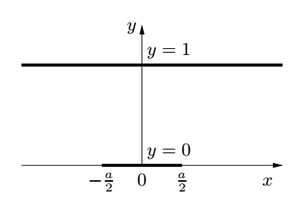
\includegraphics[scale=0.5]{images/boundary_conditions/analytic.png}
		\caption{Detector geometry for the calculation of the weighting 
			potential~\cite{pixeldetector}}
		\label{fig:analytic}
	\end{figure}

	Its exppresion is given by the following :

	\begin{equation}
		\phi_w = atan\left({\sin(\pi y)\sinh(\pi {a\over{2}})\over{\cosh(\pi x)-\cos(\pi y)\cosh(\pi {a\over{2}})}}\right)
		\label{analytic}
	\end{equation}

	\subsection{All boundaries set to zero}

\section{Applications}

	In this section we will talk about three applications of our program.
	Firstly we will talk about the simulation of a silicon detector, then the
	simulation of two cases of an helium detector, each with their own properties.

	We will compare our results with known results, and for the silicon we will also
	compare it with Weightfield, which can simulate a silicon detector.

	\subsection{Silicon detector}

		The silicon detector was the first type of detector that was implemented.

		For the application on the silicon detector, we used a serrated and rectangular detector
		(see Figure~\ref{fig:serrated_rect_geometry}) using realistic dimensions and voltage.
		In order to use the silicon type for the running of the program, the user have to specify
		it by using a macro define in the file \texttt{Constants.hpp}.

		The silicon detector uses all the features provided by the program, except the Townsend
		avalanche, which is unique to gas detectors.

		\subsubsection*{Different constants}

			In order to contextualize the results shown below, it is necessary to first set the
			different constants used in the equations of the part~\ref{equations} of this thesis.
			All the constants introduced below takes those values only for the case of a silicon
			detector, of course.

			\begin{itemize}

				\item $w = 3 eV$ : $w$ is the average energy to produce one ion-pair.
				\item $\mu_e = 1350 cm^2V^{-1}s^{-1}$ : $\mu_e$ is the mobility of the electrons
					when not considering saturation.
				\item $\mu_h = 450 cm^2V^{-1}s^{-1}$ : $\mu_h$ is the mobility of the holes (ions)
					when not considering saturation.
				\item $v_{sat} = 8,37*10^{4} ms^{-1}$ : $v_{sat}$ is the saturation velocity.

			\end{itemize}

			We do not need the values of the other constants used in part~\ref{equations} since
			those are for the Townsend avalanche which don't apply here.

			To be fully consistent, we also need the dimensions of our detector:

			\begin{itemize}

				\item Detector width $= 300 \mu m$ : The width of the detector.
				\item Strip length $= 25 \mu m$ : The length of one strip (where the potential is
					applied).
				\item Pitch $= 100 \mu m$ : The distance between the middle of a strip and the middle
					of the next one.
				\item $V_b = 100 V$ : The bias voltage applied.
				\item $V_d = 50 V$ : The depletion voltage applied (Our program don't use it, we only
					need it in Weightfield).

			\end{itemize}

		\subsubsection*{Results}

			Let's now talk about the results given by the program and let's compare them with Weightfield.

			The program \textit{Pdetect} simulate the induced current on the strips when a particle passes through it.
			For those results we are using a detector with only one strip and a particle passing vertically right in
			the middle of it, both in \textit{Pdetect} and in Weightfield, to have a better comparison. The
			Figure~\ref{fig:silicon} shows both the current simulate by \textit{Pdetect} and Weightfield.

			\begin{figure}[H]
			  \center
			  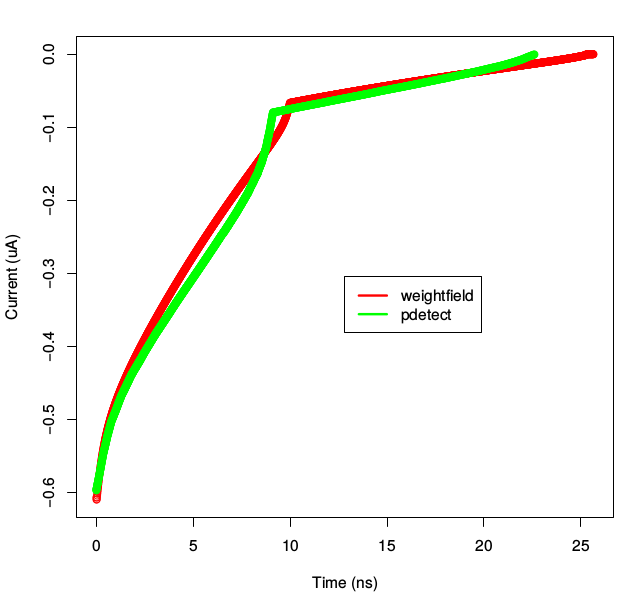
\includegraphics[scale=0.5]{images/applications/silicon_current.png}
			  \caption{Current induced by a particle in function of time, in a silicon detector.}
			  \label{fig:silicon}
			\end{figure}

			By taking a closer look, we see the total time taken for the generated ions-pair to move to the edges of the
			detector is exactly $22,6056ns$ for \textit{Pdetect} and $25,28ns$ for Weightfield. Also the maximum
			currents are respectively $-0,596511\mu A$ and $-0,606824\mu A$. Plus there are clearly some slight
			differences in the two graphs. Those differences are due to some effects featured in Weightfield
			but not in \textit{Pdetect} such as the depletion voltage or the gain.

			Indeed, the number of ions-pair generated by the pass of particle in \textit{Pdetect} and in Weightfield
			are respectively $22275$ pairs and $21222$ pairs. Such a small difference wouldn't justify the difference
			of current induced, especially since Weightfield has a bigger maximum current but less ions-pair generated.

	\subsection{Helium detector}

		The helium detector is the second type of particle detector implemented. The mechanics are basically
		the same as for the silicon detector, the detector is also a serrated and rectangular detector
		(see Figure~\ref{fig:serrated_rect_geometry}). The only real difference is the use of the Townsend
		avalanche for the the helium detector (or for any other gas detector).

		Once again the user can use the helium detector by using a macro defined in the file
		\texttt{Constants.hpp}.

		\subsubsection*{Different constants}

			Since it is another type of detector, it has its own properties and therefore the constants
			used for the silicon detector may not be used. We thus redefined the constants used in the
			equations of part~\ref{equations} for the case of helium detector and define the constants
			used for the Townsend avalanche :

			\begin{itemize}

				\item $w = 100 eV$
				\item $\mu_e = 100 cm^2V^{-1}s^{-1}$
				\item $\mu_h = 0.1 cm^2V^{-1}s^{-1}$
				\item $v_{sat} = 50 ms^{-1}$ : $v_{sat}$
				\item $p = 1 atm$ : The pressure inside the detector.
				\item $a = 3 Torr^{-1}cm^{-1}$ : A constant used in the computation of the first
					Townsend coefficient (taken from the lesson of Eduardo Cortina Gil~\cite{lphy2236}).
				\item $b = 34 VTorr^{-1}cm^{-1}$ : Another constant used in the computation of the
					first Townsend coefficient (taken from the lesson of Eduardo Cortina Gil~\cite{lphy2236}).

			\end{itemize}

			For the helium detector we will make two applications by simply changing the dimensions of
			the detector.

			The first application will use those dimensions :
			\begin{itemize}

				\item Detector width $= 5 mm$
				\item Strip length $= 0,9 cm$
				\item Pitch $= 1 cm$
				\item $V_b = 10000 V$

			\end{itemize}

			And the second application will use those :

			\begin{itemize}

				\item Detector width $= 3 cm$
				\item Strip length $= 100 \mu m$
				\item Pitch $= 1 cm$
				\item $V_b = 2000 V$

			\end{itemize}

		\subsubsection*{Results}

			For the helium detector, there are no comparisons with Weightfield since it doesn't simulate
			any gas detector. The comparisons will thus be done with known results.

			We will begin by the first case and discuss about the second later.
			The resulting current simulated by \textit{Pdetect} for the first case is shown on
			Figure~\ref{fig:helium1_unprecise} (The particle passes again vertically in the middle of
			the strip).

			\begin{figure}[H]
			  \center
			  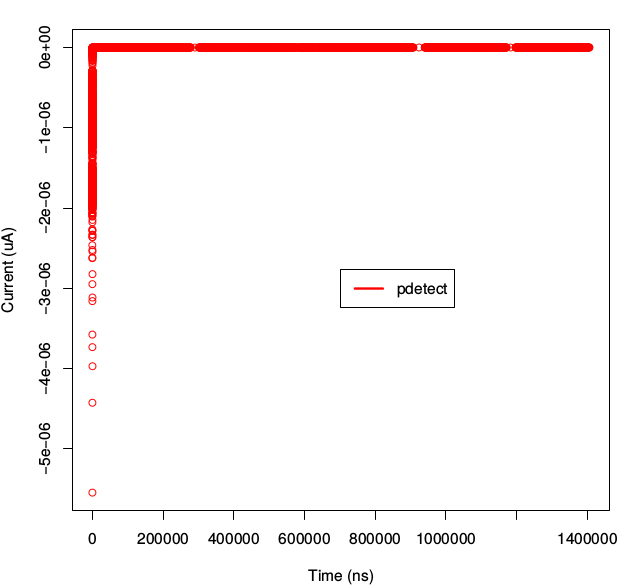
\includegraphics[scale=0.5]{images/applications/helium1_unprecise.png}
			  \caption{Current induced by the ions-pair in function of time, in the first case of helium detector.}
			  \label{fig:helium1_unprecise}
			\end{figure}

			It seems, on the graph, to have a peak of current when the particle deposit the charges in the
			detector which fade almost instantly. Actually that is not what happens. This peak of current
			is the result of the electrons moving towards the detector to reach the anode. But since those
			electrons are way quicker than the holes (almost a thousand times quicker), they will reach the
			anode long before the holes reach the cathode. Once the electrons are all at the anode, only holes
			remain in the detector. Due to their slowness, they induce a current so small compare to the
			current that was induced by the electron that it seems on the graph to have no current.

			The Figure~\ref{fig:helium1_precise} shows the current induced only by the electrons (by simply zooming
			on this part in the Figure~\ref{fig:helium1_unprecise}).

			\begin{figure}[H]
			  \center
			  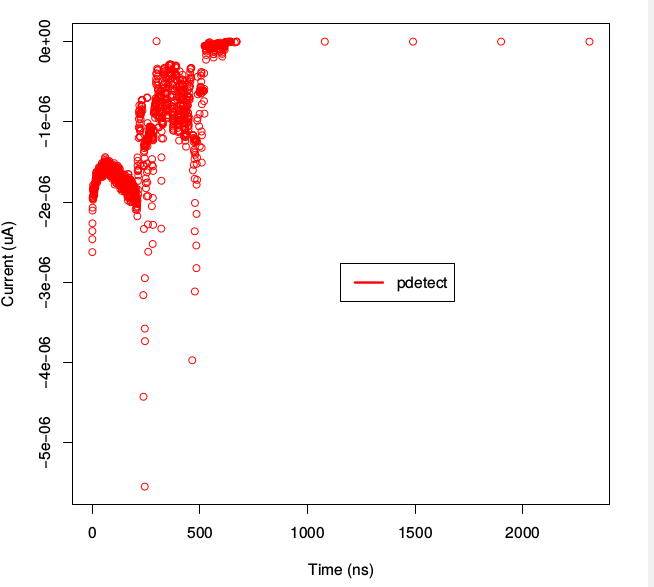
\includegraphics[scale=0.5]{images/applications/helium1_precise.png}
			  \caption{Current induced by the electrons in function of time, in the first case of helium detector.}
			  \label{fig:helium1_precise}
			\end{figure}

			Now it is clear that this peak of current didn't fade instantly. Instead, there is now a weird-shaped
			graph that has nothing to do with the one of the silicon detector (Figure~\ref{fig:silicon}). Why?

			This is due to the Townsend avalanche. While the electrons are moving toward the anode and some of them stop
			(because they've reached it), other ions-pair are formed by this Townsend avalanche, if the electric field is
			high enough. Therefore the new holes and electrons formed will contribute to the current. The resulting current
			will thus increase, as shown on Figure~\ref{fig:helium1_precise}, around the times of $250ns$ or $500ns$.

			The threshold value of the electric field needed for the Townsend avalanche to occur is $~10^6V/m$. With the
			dimensions of the detector used in the first application, the electric field near the anode is around
			$2*10^6V/m$, enough to see the Townsend avalanche occurs.

			The graph also shows a very small current, of the order of $-10^{-6}\mu A$. This is simply due to the little
			amount of ions-pair generated when the particle passes through the detector. Indeed, with the dimensions of the
			first application of helium detector, the particle generates only $4$ ions-pair ($3,9$ to be precise). The detector
			being half a centimeter thick, the particle thus generates between $7,8$ and $8$ ions-pair per centimeter.
			This result is totally realistic, using the lesson of Eduardo Cortina Gil~\cite{lphy2236}, we see the theoretical
			number of ions-pair in a helium detector is $7,8$ ions-pair per centimeter. We can therefore assume that the
			results given by \textit{Pdetect} are accurate.

			Let's now talk about the second case of helium detector. The graph of the induced current is shown on
			Figure~\ref{fig:helium2_unprecise}.

			\begin{figure}[H]
			  \center
			  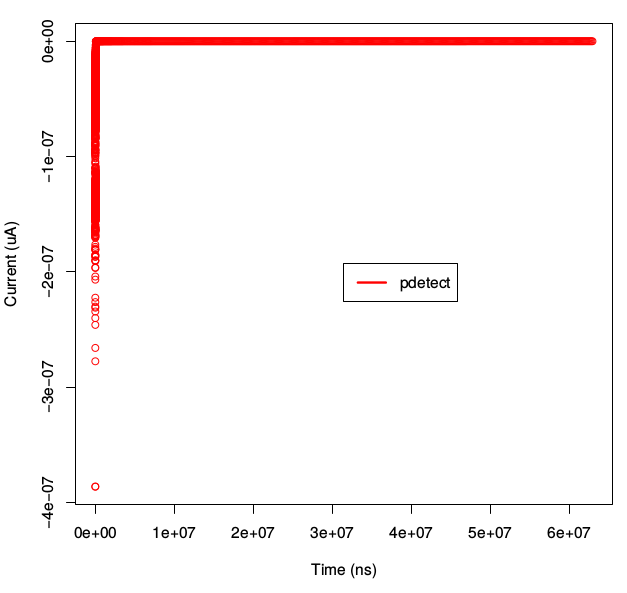
\includegraphics[scale=0.4]{images/applications/helium2_unprecise.png}
			  \caption{Current induced by the ions-pair in function of time, in the second case of helium detector.}
			  \label{fig:helium2_unprecise}
			\end{figure}

			Once again the graph isn't very explicit due to the slowness of the holes compared to the electrons.
			Figure~\ref{fig:helium2_precise} shows the current induced by the electrons only (once again, it's only
			a zoom from from Figure~\ref{fig:helium2_unprecise}).

			\begin{figure}[H]
			  \center
			  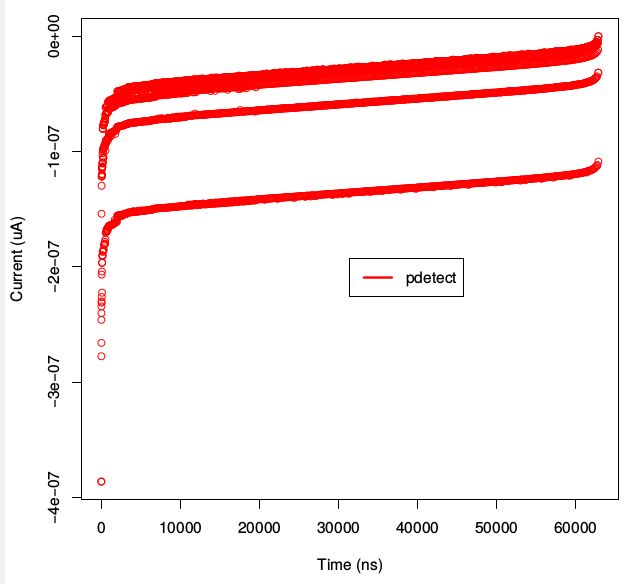
\includegraphics[scale=0.4]{images/applications/helium2_precise.png}
			  \caption{Current induced by the electrons in function of time, in the second case of helium detector.}
			  \label{fig:helium2_precise}
			\end{figure}

			The aspect of the graph on Figure~\ref{fig:helium2_precise} has nothing to do with the others. This is due
			to the dimension of the detector used in this application. Indeed, the strip is so small compared to the
			detector that the electric field it generates is really low (Figure~\ref{fig:electric_field} shows the electric
			field inside the detector). Therefore the charges (holes and electrons) are moving slowly towards the edges of
			the detector. Since they move slowly, the induced current is quite small. After a certain time (an iteration
			of the program for example), the electrons are closer to the anode (only the electrons induce a relevant current),
			where the electric field grow higher rapidly. The electrons have then a bigger velocity and induced a bigger
			current. Again after some iterations, the closest electrons, which generate the higher current, reach the anode.
			The next few electrons being further will induce a little current and the cycle goes on. This is why there are
			different \"branches\" on the graph.

			\begin{figure}[H]
			  \center
			  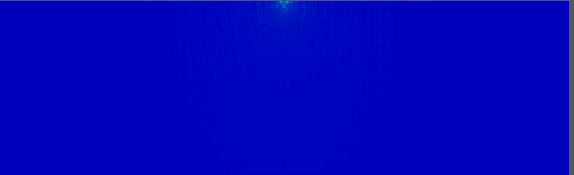
\includegraphics[scale=0.4]{images/applications/electric_field.png}
			  \caption{Electric field inside the detector (Top quarter of the detector)}
			  \label{fig:electric_field}
			\end{figure}

			In this case, due to the low electric field, the Townsend avalanche don't occurs. This is why the graph doesn't
			look like the first one and why the current is so slow (the maximum current is $-3,86328*10^{-7}\mu A$) even though
			there are much more ions-pair generated by the particle, $23$ ions-pair are generated along its path (the theoritical
			number is $23,4$ ions-pair for three centimeters).

\section{Future work}

There are a lot of ways to improve and extend the developed software.

Authors highlight five new features that could be introduced. Firstly, the
computation of the current for the
rectangular geometry with circular holes could be implemented quite easily.
Secondly, additional physical effect
could be implemented such as the \textit{Geiger avalanche}. Thirdly,
additional 2D geometries could be introduced such as
rectangular potential sources but with gaussian curves at their corners.
Fourthly, the software can be extended to handle both 2D and 3D geometries.
Fifthly, a graphic user interface could be developed to ease the usage of the
software.

Furthermore, since the passage to 3D geometries will slow down the computations,
it may become interesting to modify the \texttt{deal.ii} code in the
\texttt{LaplaceSolver} class in order to run the software on clusters.
Research could also be performed on how to efficiently parallelize the
computation of the current among several CPU cores (the finite element method
is multithreaded but the current computation is not for now) or among nodes of a cluster.
Another performance improvement would be to offload some computations on
Graphics Processing Unit.

\section*{Conclusion}

\newpage

\bibliographystyle{plain}
\bibliography{report.bib}

\end{document}
